% figures/screening_pipeline.tex
% Standalone — compile with:
%   xelatex -interaction=nonstopmode screening_pipeline.tex
\documentclass[tikz, border=4pt]{standalone}

%% ---------- Packages ----------
\usepackage{fontspec}          % XeLaTeX font selection
\usepackage{xcolor}
\usepackage{tikz}
\usetikzlibrary{positioning, shapes.geometric, arrows.meta}

%% ---------- Colours ----------
\definecolor{colorA}{HTML}{2E86AB}   % Stage 1 — blue
\definecolor{colorB}{HTML}{A23B72}   % Stage 2 — plum
\definecolor{colorC}{HTML}{F18F01}   % Stage 3 — amber
\definecolor{colorD}{HTML}{3B1F2B}   % Synthesis — dark
\definecolor{colorGray}{HTML}{BFC0C0}
\definecolor{colorReject}{HTML}{C1292E}

%% ---------- TikZ node styles (colour fills) ----------
\tikzset{
  flowColorA/.style    = {fill=colorA!15,    draw=colorA,    text=colorA!60!black},
  flowColorB/.style    = {fill=colorB!15,    draw=colorB,    text=colorB!60!black},
  flowColorC/.style    = {fill=colorC!15,    draw=colorC,    text=colorC!60!black},
  flowColorD/.style    = {fill=colorD!15,    draw=colorD,    text=colorD!60!black},
  flowColorGray/.style = {fill=colorGray!30, draw=colorGray!80!black, text=black},
  flowColorReject/.style = {fill=colorReject!10, draw=colorReject, text=colorReject!80!black},
}

%% ---------- Arrow styles ----------
\tikzset{
  arrowMain/.style   = {-{Stealth[length=7pt]}, thick,        draw=black!70},
  arrowReject/.style = {-{Stealth[length=6pt]}, thick, dashed, draw=colorReject},
}

%% ---------- Document ----------
\begin{document}
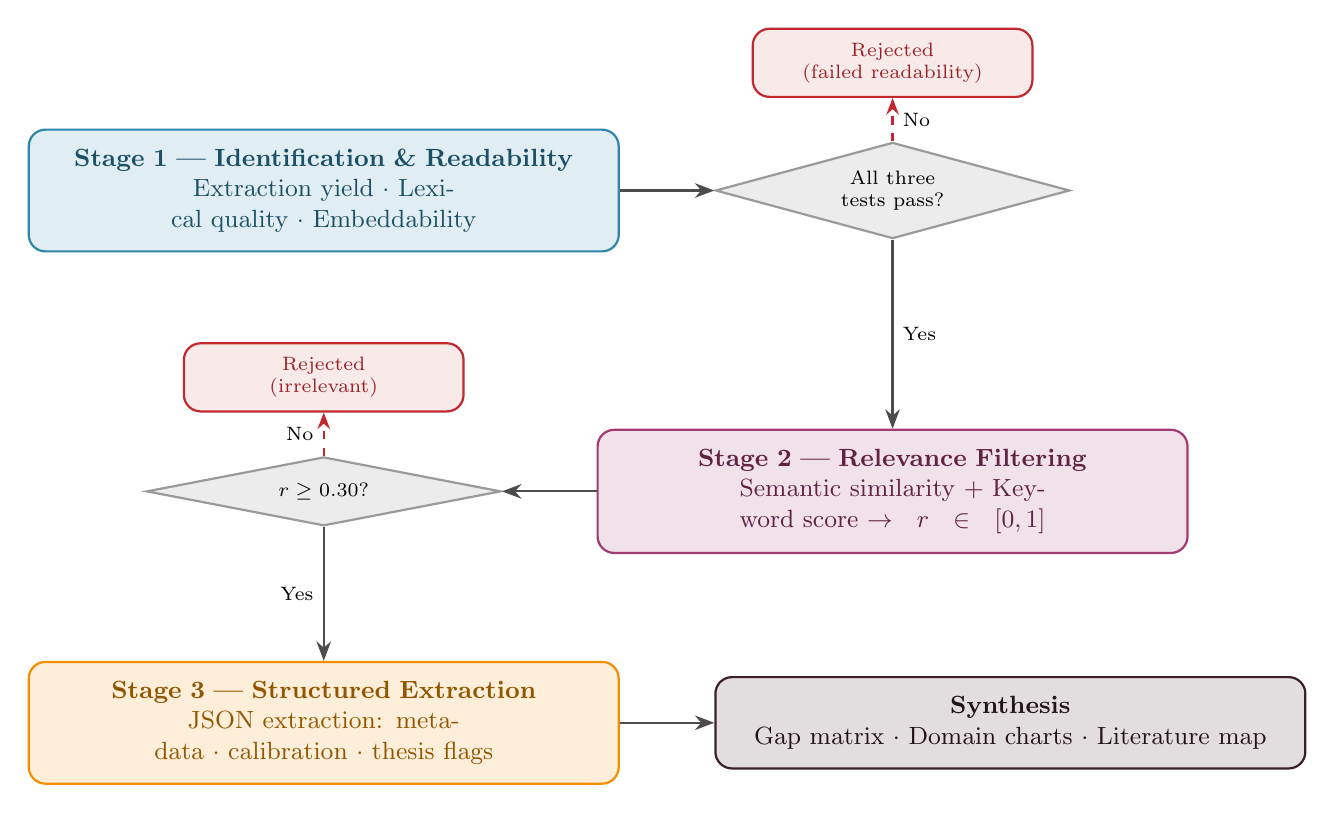
\begin{tikzpicture}[
    box/.style      = {rectangle, rounded corners=6pt, thick,
                       text width=7.0cm, align=center,
                       minimum height=0.85cm, inner sep=7pt,
                       font=\small},
    decision/.style = {diamond, thick, aspect=2.5,
                       minimum width=4.5cm, minimum height=0.7cm,
                       align=center, font=\scriptsize, inner sep=2pt},
    rej/.style      = {rectangle, rounded corners=6pt, thick,
                       text width=3.2cm, align=center,
                       minimum height=0.75cm, inner sep=5pt,
                       font=\scriptsize},
  ]

  %% --- Row 1 : left -> right ---
  \node[box, flowColorA] (s1)
    {\textbf{Stage 1 --- Identification \& Readability}\\
     Extraction yield $\cdot$ Lexical quality $\cdot$ Embeddability};

  \node[decision, flowColorGray, right=1.2cm of s1] (d1)
    {All three\\tests pass?};

  %% --- Row 2 : right -> left ---
  \node[box, flowColorB, below=2.4cm of d1] (s2)
    {\textbf{Stage 2 --- Relevance Filtering}\\
     Semantic similarity $+$ Keyword score $\to r \in [0,1]$};

  \node[decision, flowColorGray, left=1.2cm of s2] (d2)
    {$r \geq 0.30$?};

  %% --- Row 3 : left -> right ---
  \node[box, flowColorC, below=1.7cm of d2] (s3)
    {\textbf{Stage 3 --- Structured Extraction}\\
     JSON extraction: metadata $\cdot$ calibration $\cdot$ thesis flags};

  \node[box, flowColorD, right=1.2cm of s3] (out)
    {\textbf{Synthesis}\\
     Gap matrix $\cdot$ Domain charts $\cdot$ Literature map};

  %% --- Rejection nodes ---
  \node[rej, flowColorReject, above=0.55cm of d1] (r1)
    {Rejected\\(failed readability)};

  \node[rej, flowColorReject, above=0.55cm of d2] (r2)
    {Rejected\\(irrelevant)};

  %% --- Main snake flow ---
  \draw[arrowMain] (s1) -- (d1);
  \draw[arrowMain] (d1) -- node[right, font=\scriptsize]{Yes} (s2);
  \draw[arrowMain] (s2) -- (d2);
  \draw[arrowMain] (d2) -- node[left,  font=\scriptsize]{Yes} (s3);
  \draw[arrowMain] (s3) -- (out);

  %% --- Rejection branches ---
  \draw[arrowReject] (d1) -- node[right, font=\scriptsize]{No} (r1);
  \draw[arrowReject] (d2) -- node[left,  font=\scriptsize]{No} (r2);

\end{tikzpicture}
\end{document}
